\chapter{Umsetzung}
\label{ch:implementation}
In diesem Kapitel wird die prototypische Verprobung des Anwendungsfalls vorgestellt; dazu werden die Architektur und der Aufbau der Implementierung aufgezeigt. Das Vorgehen für das Testing und das Deployment werden vorgestellt und Betrachtungen zu Datenschutz und Privatsphäre durchgeführt. Die Anforderungserfüllung wird geprüft und für alle \ac{DLT}-relevanten Anforderungen im Detail untersucht. Im Fokus dieser Betrachtungen steht die Eignung von \ac{DLT} für den \ac{IOT}-Anwendungsfall.

\section{Architektur und Aufbau}
\label{sec:implementation:poc:architecture}
Die prototypische Verprobung des Anwendungsfalls wurde auf Basis der Ethereum-Blockchain umgesetzt. Die Gesamtarchitektur wurde mittels \ac{UML}-Komponentendiagramm modelliert und ist in Abbildung \ref{fig:chapter07:architecture} zu sehen.

\begin{figure}[h]
 \centering
 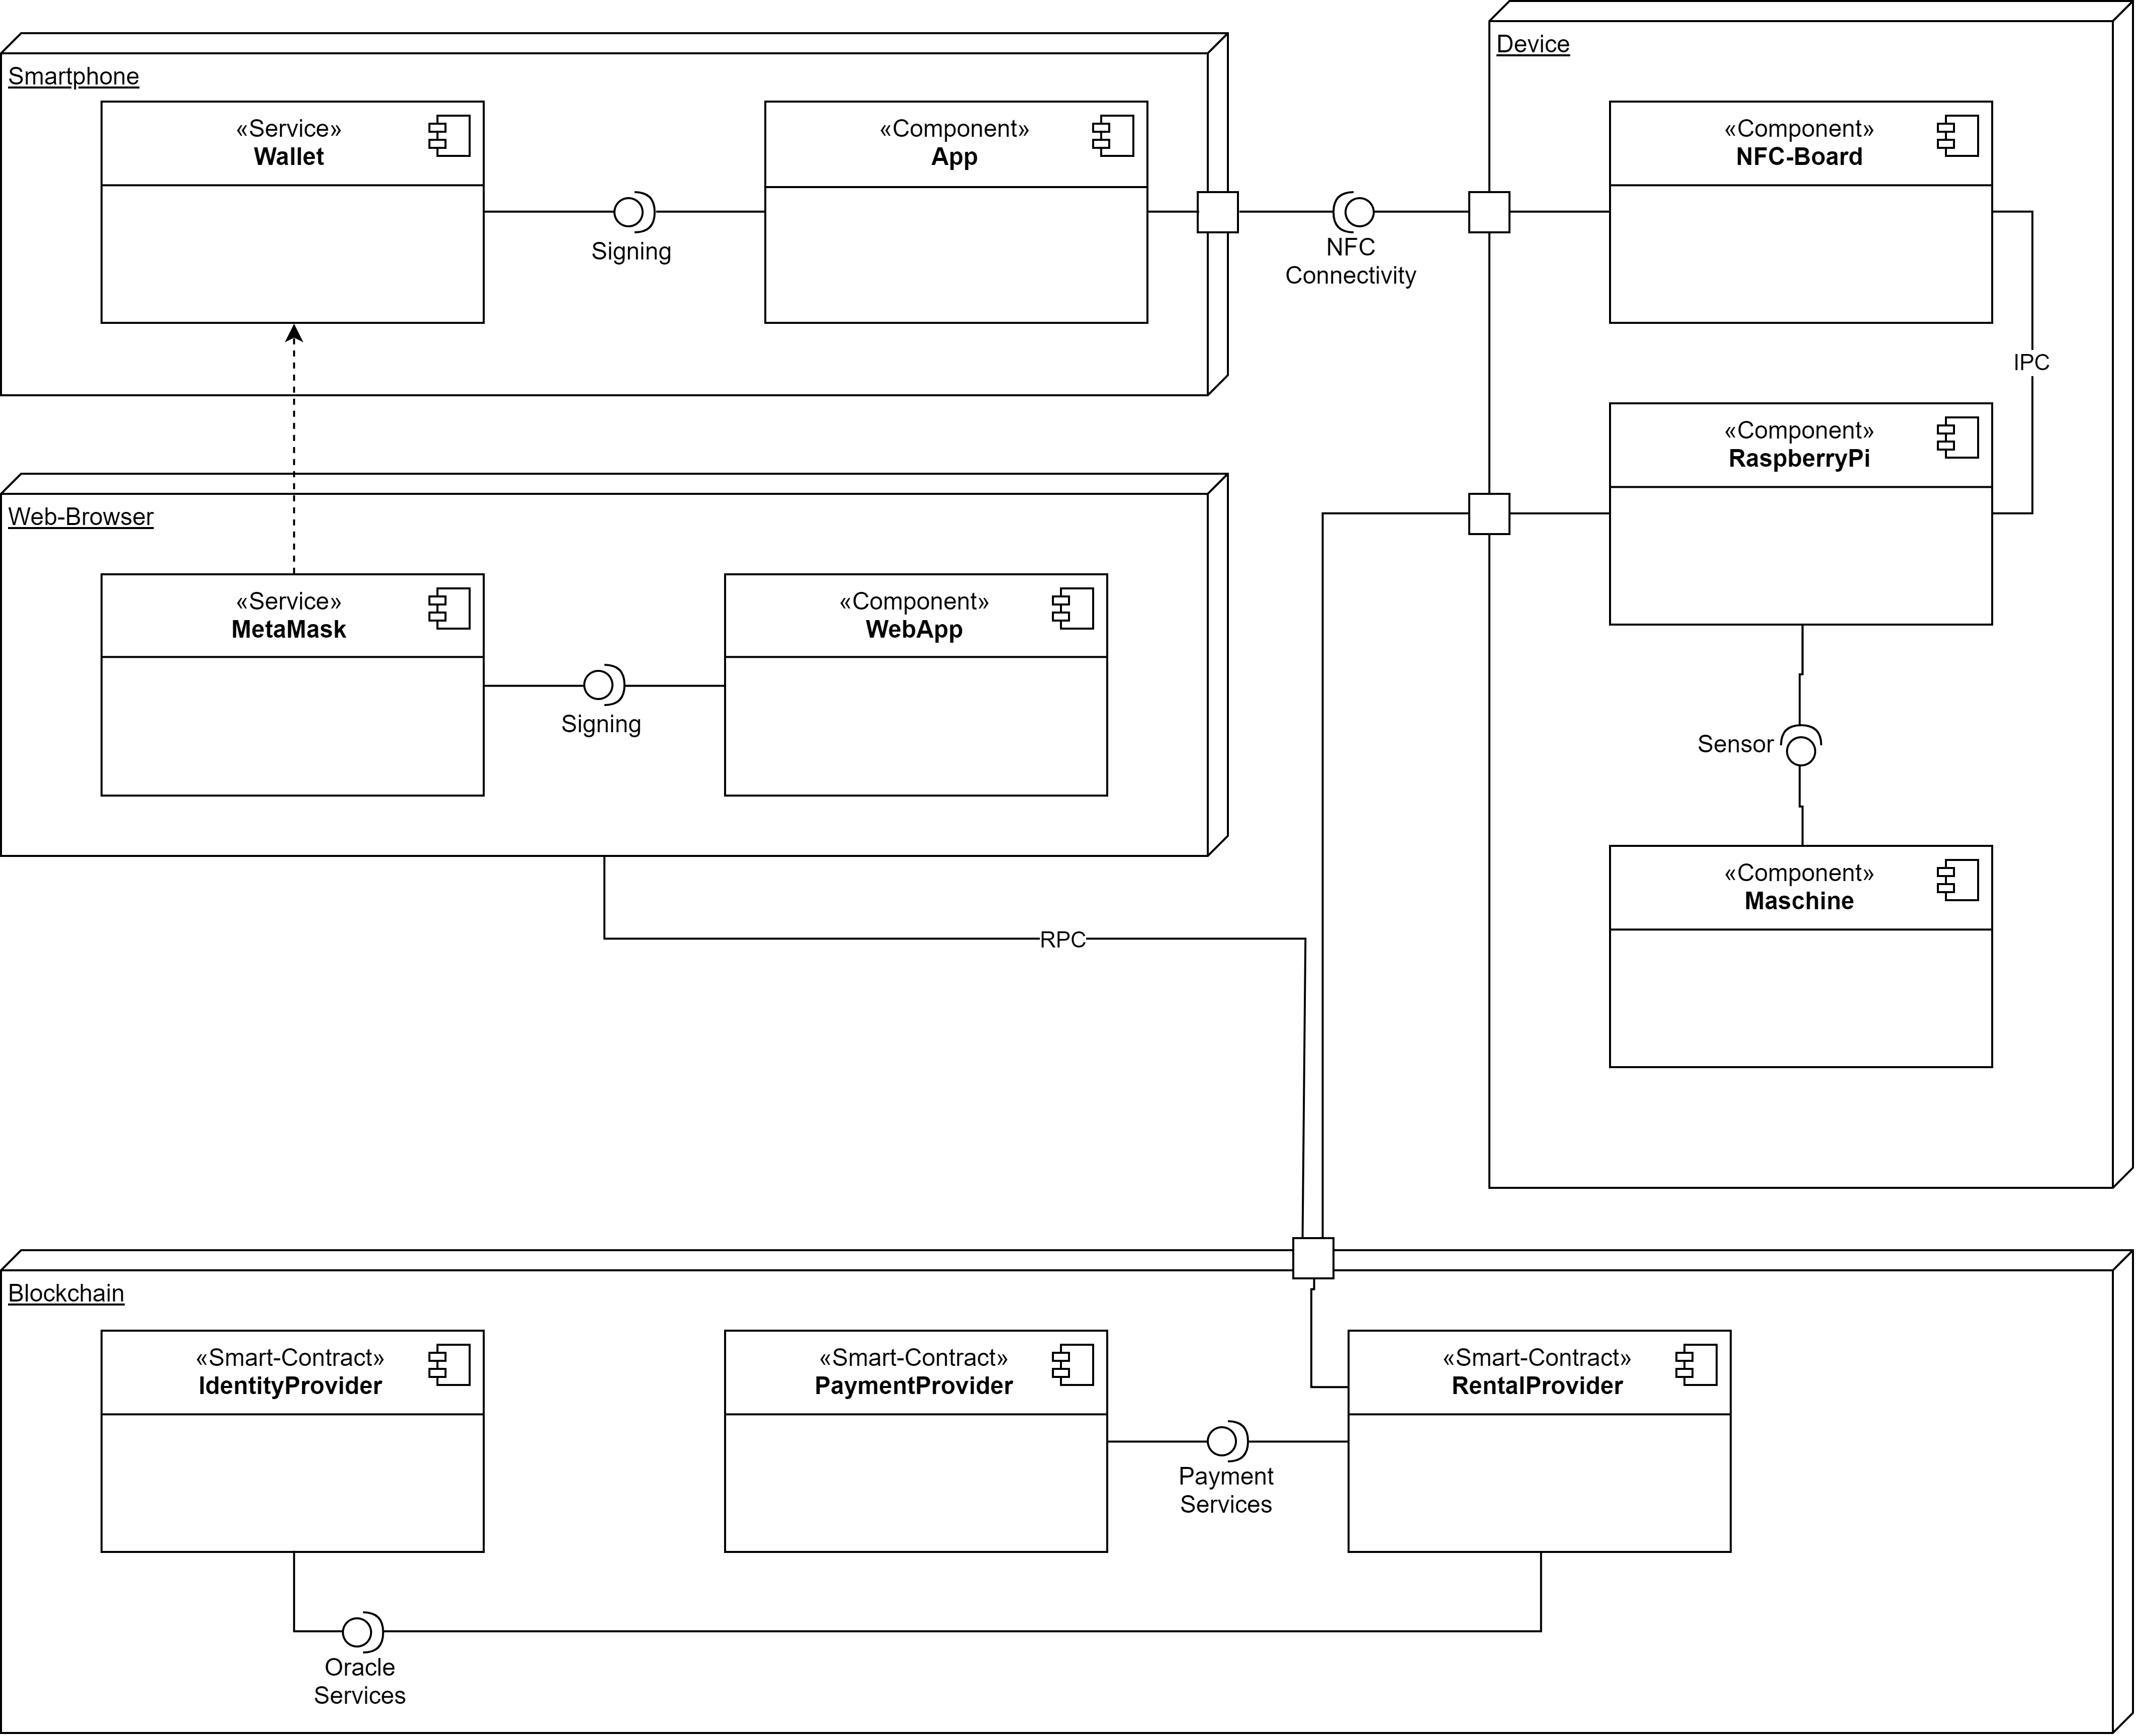
\includegraphics[width=1.0\textwidth]{gfx/Architecture.png}
 \caption{Architektur als UML-Komponentendiagramm}
 \label{fig:chapter07:architecture}
\end{figure}

Die Umsetzung wurde zunächst so vorgenommen, dass ein Benutzer durch ein Unternehmen dargestellt wird. Die Mitarbeiter eines Unternehmens, die den Kaffee konsumieren, sind vorerst nicht als eigenständige Akteure auf der Plattform tätig und agieren über ihr Unternehmen mit den Geräten.\\
Jeder Benutzer besitzt eine Wallet, auf die nur er mittels des passenden Private-Keys Zugriff hat. Diese Wallet wird benötigt, um den Benutzer zu identifizieren und Bezahlvorgänge durchzuführen. Über das Browser-Plugin Metamask\footnote{Verbreitetes Ethereum-Wallet Plugin für Chrome und Firefox} kann der Benutzer Zahlungen innerhalb der Web-App autorisieren und sich dort anmelden. Die Web-App wurde als React-Anwendung entwickelt und wird im Browser ausgeführt. Per \ac{RPC} ist sie in der Lage, auf Informationen innerhalb der Blockchain zuzugreifen und mit Smart-Contracts zu interagieren. Es wurden drei Smart-Contracts entwickelt: Der IdentityProvider fungiert als Oracle-Service und hält Informationen über Identitäten und deren Rollen. Der PaymentProvider ist zuständig für die Zahlungsabwicklungen und hält Payment-Channel und Zahlungshistorien der Verträge. Letztere werden über den RentalProvider abgebildet, angefragt und verwaltet. Der zentrale Gegenstand eines Mietvertrages im vorliegenden Anwendungsfall ist die Kaffeemaschine. Diese besitzt interne Sensoren, um über den aktuellen Zustand zu informieren. Die Maschine als Ganzes wird ergänzt durch ein NFC-Modul und einen daran angeschlossenen Raspberry-Pi Einplatinencomputer. Dieser übernimmt die Kommunikation mit den Geräte-internen Sensoren, dem NFC-Modul und der Blockchain und stellt damit das Herzstück des Geräts dar. Mittel eines Smartphones ist der Benutzer in der Lage, mit der Kaffeemaschine per \ac{NFC} zu kommunizieren\footnote{Voraussetzung hierfür ist ein funktionsfähiger NFC-Chip im Smartphone}. Die dazu notwendige App greift zur Identifikation und Autorisierung von Bezahlvorgängen auf das hinterlegte Wallet zu. Es handelt sich dabei um das gleiche Wallet, welches auch in der Web-App hinterlegt wurde und auf welches mittels Metamask zugegriffen wird.

\section{Deployment}
\label{sec:implementation:poc:deployment}
Die Smart-Contracts wurden auf dem öffentlichen Kovan-Testnet deployed. Es handelt sich bei Kovan um ein \ac{PoA}-Netzwerk, das zu Testzwecken ausgewählt wurde, da die Blockzeit bei nur etwa vier Sekunden (vgl. \url{https://kovan.etherscan.io/}) liegt. Das Ropsten-Testnet, welche auf \ac{PoW} basiert und dem Mainnet am ähnlichsten ist, benötigt für das Minen eines Blocks etwa 15 Sekunden\footnote{Im Laufe der Entwicklung kam es vor, dass Transaktionen teils mehrere Minuten benötigten, bis sie durch das Netzwerk bestätigt wurden. Deshalb wurde zunächst auf Kovan umgeschwenkt.}. Tabelle \ref{tab:addresses} listet die Adressen auf, unter denen die Smart-Contracts erreichbar sind.

\begin{table}[]
\begin{tabular}{@{}ll@{}}
\toprule
\textbf{Smart-Contract} & \multicolumn{1}{c}{\textbf{Kovan-Adresse}} \\ \midrule
Rental-Provider & 0xf25F1F12630158d963a9609950C3e379c65617dA \\
Identity-Provider & 0xA17351BfA16dAE1FD285e11AcC00882Eb459C7cb \\
Payment-Provider & 0x7d17DA28604A7bB2E121D634012C086A6BbF6E2e \\ \bottomrule
\end{tabular}
\caption{Adressen der Smart-Contracts auf dem öffentlichen Kovan Testnet}
\label{tab:addresses}
\end{table}

Das Frontend wurde per Heroku deployed und ist unter \url{https://dlt-iot-synergy.herokuapp.com/} erreichbar. Nach eigenen Angaben handelt es sich bei Heroku um eine "Platform as a Service (PaaS), die Entwickler dazu befähigt, Anwendung vollumfänglich in der Cloud zu bauen und zu betreiben". Mittels Git push-Befehl kann aus dem lokalen Repository der Code in eine Heroku-App deployed werden.

\begin{figure}[h]
 \centering
 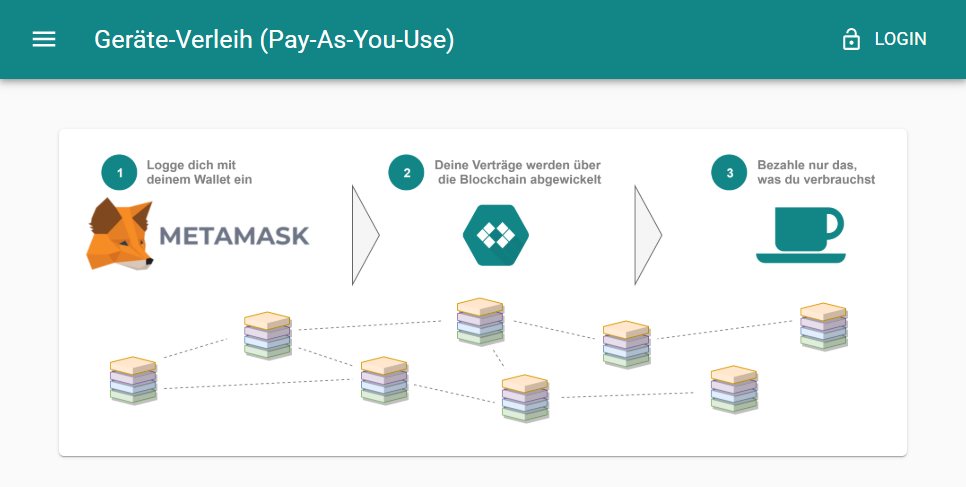
\includegraphics[width=1.0\textwidth]{gfx/screenshots/frontend.PNG}
 \caption{Frontend deployed mittels Heroku}
 \label{fig:chapter07:frontend}
\end{figure}

Die Smartphone-App wurde lokal auf einem Android-Device von Samsung installiert.

\section{Testaufbau}
\label{sec:implementation:poc:testing}
Für Smart-Contracts auf Ethereum-Basis existiert die Truffle-Suite, die ein umfangreiches Toolset für die Entwicklung und das Testen von Smart-Contracts bereitstellt. Der Entwicklungsprozess wird durch eine lokale Blockchain-Umgebung vereinfacht, die das Deployment und Testing beschleunigt. Mittels Unit-Tests wurde sichergestellt, dass die Funktionalität gemäß den Anforderungen gegeben ist. Die Testabdeckung wurde durch das Tool solidity-coverage überprüft, die Ergebnisse werden in Abbildung \ref{fig:chapter07:coverage} dargestellt. Die Grafik zeigt die prozentuale und absolute Abdeckung von Statements, Funktionen und Code-Zeilen an.

\begin{figure}[h]
 \centering
 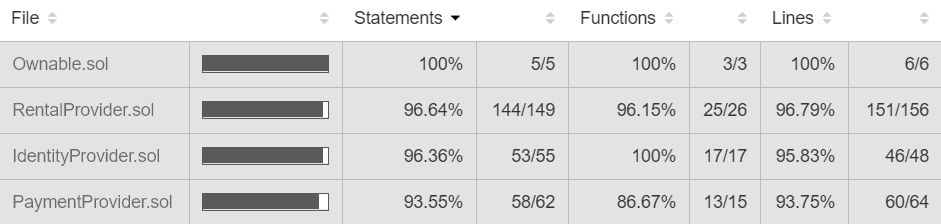
\includegraphics[width=1.0\textwidth]{gfx/coverage.png}
 \caption{Testabdeckung der Solidity Smart-Contracts}
 \label{fig:chapter07:coverage}
\end{figure}

\ac{E2E}-Tests wurden manuell durchgeführt: Alle Bestandteile der gesamten Anwendung wurden gestartet und der Anwendungsfall Schritt für Schritt durchgeführt. Aus Benutzersicht konnten alle Funktionalitäten erfolgreich getestet werden. Das Erstellen und Abschließen von Mietverträgen über die Web-App erfolgte ebenso wie die Abrechnung mittels Smartphone reibungslos.


\section{Anforderungsumsetzung}
\label{sec:implementation:requirements}
In Kapitel \ref{sec:requirements:transfer} wurden die zuvor identifizierten Anforderungen in \ac{DLT}-Spezifika übersetzt, um für die darauffolgende Auswahl eines geeigneten \ac{DLT}s überprüfbar zu sein. Diese lauteten:
\begin{itemize}
  \item Smart-Contracts
  \item Oracle-Services
  \item Zahlungsmittel
  \item Asynchronität
  \item Performanz
  \item Verschlüsselung
\end{itemize}
Im Folgenden werden diese überprüft, ob und inwieweit den Anforderungen gerecht werden konnte.

\subsection{Smart-Contracts}
\label{subsec:implementation:requirements:smart_contracts}
Die implementierten Smart-Contracts wurden nach bestem Wissen und Gewissen umgesetzt. Damit ein Smart-Contract rechtskonform agiert und um die Vertragslogik nach geltendem deutschen Recht korrekt abzubilden, bedarf es ausführlicher rechtlicher Beratung durch entsprechende Experten und Anwälte. Dieser zeitaufwändige Prozess wurde im Rahmen dieser Arbeit nicht durchgeführt. Bei einer Implementierung, die über die Machbarkeitsstudie hinausgeht und produktiv eingesetzt werden soll, muss dieser Punkt berücksichtigt werden. Damit wurde die Anforderung A1.3.2 nicht erfüllt.\\
Das Anpassen der Smart-Contracts aufgrund von Vertragsänderung oder ähnlichen Anpassungen wurde durch die Anforderung A1.3.8 gefordert. Sie beschreibt, dass Verträge im Nachhinein aktualisierbar sein müssen. Die Vertragslogik wurde mittels Smart-Contract umgesetzt: Einmal in der Blockchain gespeichert, sind Daten nicht mehr veränderlich. Es gibt dennoch Möglichkeiten, einen benötigten Mechanismus einzubauen, um die Verträge im Nachhinein anzupassen. Dazu kann man sich sogenannter Proxy-Smart-Contracts bedienen. Die Grundidee dabei ist, wie in einem Netzwerk ein zentrales Eingangstor zu haben, welches fest definiert ist und sich später nicht mehr ändert. Dieser Proxy verweist dann auf die jeweils aktuelle Version des benötigten Smart-Contracts. Ändert sich der Code durch Vertragsänderungen oder sonstige Updates, kann die aktualisierte Version in die Blockchain transferiert werden. Anschließend wird dem Proxy die Adresse des neuen Contracts mitgeteilt. Bei Anfragen an den Proxy leitet dieser den Anfragenden fortan an den neuen Vertrag weiter (der alte Vertrag bleibt dennoch weiterhin bestehen). Diese Umsetzung wurde im Zuge dieser Masterarbeit nicht geleistet, da die Umsetzung dieses Ansatzes viel Zeit und Aufwand benötigt, um die gewünschten Funktionalitäten zuverlässig zu implementieren. Da diese Arbeit als Machbarkeitsstudie aufgebaut wurde, wurde an dieser Stelle auf die Implementierung verzichtet. Es sei auf das \ac{SDK} und die auditierten Smart-Contracts von OpenZepplin (\url{https://openzeppelin.com/}) verwiesen; dort wird ein umfangreiches Toolset zur Entwicklung robuster Smart-Contracts angeboten sowie Templates bereitgestellt, die das Upgrade-Management eines Smart-Contracts übernehmen. Die Nicht-Umsetzung dieser Anforderung verhindert nicht das Aufzeigen der generellen Machbarkeit.\\

\subsection{Oracle-Services}
\label{subsec:implementation:requirements:oracle}
Der Identity-Provider Smart-Contract wurde als Oracle Smart-Contract implementiert. Er hält Informationen zu Identitäten und Rollen. Diese Informationen werden nach dem Deployment außerhalb des Blockchain-Netzwerkes generiert und durch den Eigentümer des Smart-Contracts durch onchain Transaktionen den Identity-Provider progagiert. Ab diesem Zeitpunkt fungiert der Smart-Contract als Oracle und kann durch andere Smart-Contracts nach den gespeicherten Informationen angefragt werden.\\
Das Aktualisieren und Entfernen von Informationen obliegt dem Besitzer des Smart-Contracts und ist als Sicherheitsmechanimus angedacht. Somit kann kein Dritter falsche Informationen oder Duplikate an das Oracle senden. Dieser Aufbau erfordert allerdings ein hohes Maß an Vertrauen gegenüber dem Oracle-Ersteller; da es sich allerdings um den Hersteller selbst handelt und dieser auch Besitzer der \ac{IOT}-Geräte ist, kommt es im vorliegenden Anwendungsfall zu keinen Vertrauensproblemen. Wie bereits im Grundlagenkapitel (vgl. Kap. \ref{subsec:fundamentals:dlt:smartcontracts}) aufgezeigt, können auch mehrere Oracles verschiedener Anbieter parallel existieren, um den dezentralen Charakter der Anwendung zu stärken. Die vorgenommene Implementierung könnte auch derart erweitert werden, dass mehrere Eigentümer gemeinsam für die bereitgestellten Informationen verantwortlich sind und diese gemeinsam pflegen und aktualisieren.

\subsection{Zahlungsmittel}
\label{subsec:implementation:requirements:payment}
Mit der Umsetzung auf der Ethereum-Plattform können Zahlungen mittels Ether abgewickelt werden. Darüber hinaus existieren Implementierung auf Ether-Basis, sogenannte Token, die ebenfalls als Zahlungsmittel genutzt werden können. Um den massiven Kursschwankungen von Ethereum entgegenzuwirken, können sogenannte Stable-Coins eingesetzt werden, die durch besondere Algorithmen oder Einlagenabsicherung die Schwankungen unterbinden. Der Einfachheit halber wurde in dieser Arbeit Ether als Zahlungsmittel eingesetzt.\\

Eine zentrale Fragestellung, die sowohl Betreiber als auch Benutzer der Plattform interessiert, lautet: Was kostet die Nutzung? Die folgenden Berechnungen wurden auf Basis des Wechselkurses vom 06.02.2020 für 196.04€ pro 1ETH durchgeführt.\\
Der GAS-Preis\footnote{GAS ist eine Ethereum-interne Einheit, mit der Rechenoperationen gemessen werden.} ist ein Hebelpunkt, mit dem die Bestätigungsdauer von Transaktionen beeinflusst werden kann. Setzt man diesen auf einen hohen Wert (beispielsweise größer als 12 GWEI\footnote{1 WEI ist die kleinste Währungseinheit, mit der beispielsweise GAS bezahlt wird. 1GWEI = 1 Giga-WEI oder $ 10^{9} $WEI oder $ 10^{-9} $ETH}), so werden Miner diese Transaktion bevorzugt behandeln, da sie an ihr entsprechend mehr verdienen. Somit hängt die Performanz direkt an den Transaktionskosten, wobei eine natürliche Grenze vorliegt: Wie der Abbildung \ref{fig:chapter07:blocktime} zu entnehmen ist, liegt die Block-Zeit von Ethereum bei etwa 15 Sekunden. Unabhängig vom bezahlten GAS-Preis kann diese Grenze nicht unterschritten werden, da immer mindestens eine Blockdauer vergehen muss, damit die Transaktion in den Ledger aufgenommen wird.

\begin{figure}[h]
 \centering
 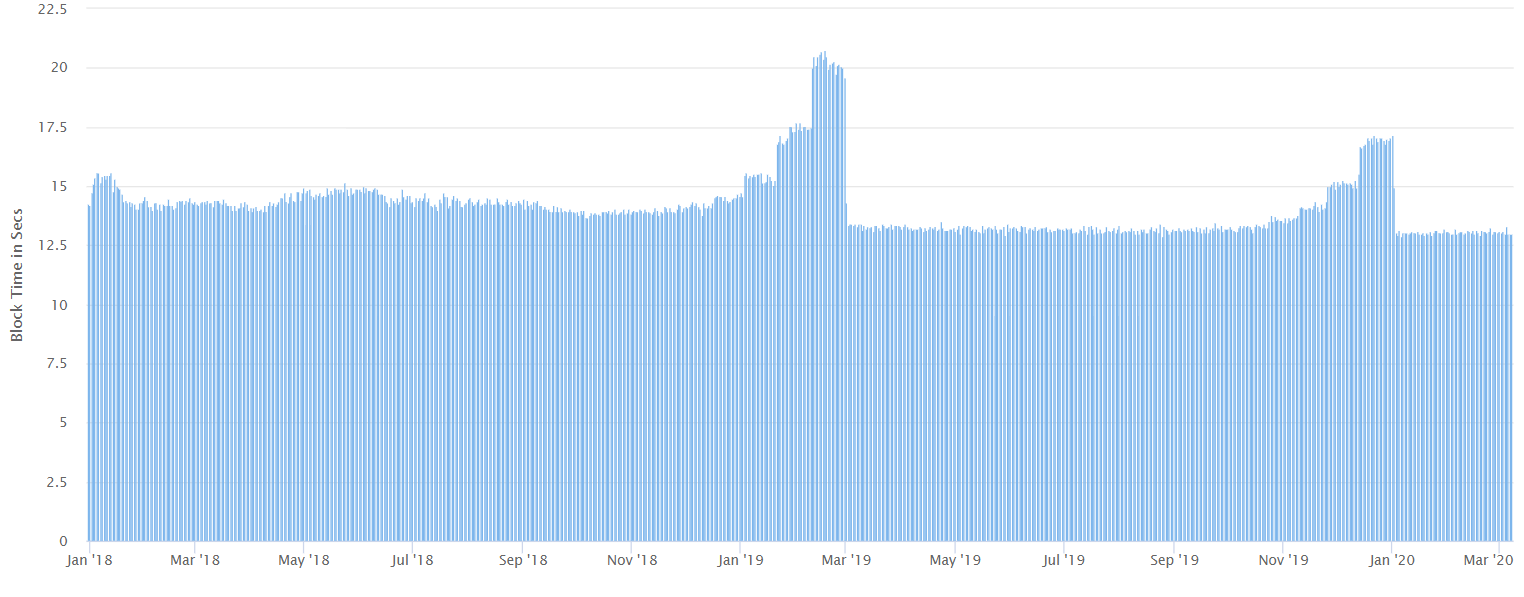
\includegraphics[width=1.0\textwidth]{gfx/screenshots/blocktime_ETH.PNG}
 \caption{Blockzeit von Ethereum innerhalb des letzten Jahres, Quelle: \url{etherscan.io}}
 \label{fig:chapter07:blocktime}
\end{figure}

Um eine einheitliche Kalkulation vorzunehmen, wird in den folgenden Berechnungen ein GAS-Preis von 5 GWEI angenommen; dieser Preis wurde auch für das Testen eingesetzt. Die Korrelation zwischen Preis und Performanz wurde bereits erläutert. Wird eine erhöhte Performanz benötigt, so kann dies mit einem höheren GAS-Preis erzielt werden.\\
In Tabelle \ref{tab:costs} ist zu sehen, dass die Kosten für einen Benutzer zur Vertragserzeugung bei 35 Cent liegen. Die Transaktionsgebühr zum Aufladen des Payment-Channels ist mit drei Cent pro Aufladung verschwindend gering. Aus der Perspektive des Herstellers liegen die Kosten pro Vertragsinteraktion etwas höher bei 42 Cent zur Erstellung und 15 Cent für das Einlösen einer Quittung. Bei einer Endausbaustufe von 400.000 Benutzern und 10.000 Maschinen beläuft sich die jährliche Gebühr für das Einlösen der Quittungen (unter der Annahme, dass alle Quittungen einmal pro Woche eingelöst werden) auf 78.000€ bei einem Umsatz von 82.000.000€. Zu Vertragsbeginn fallen einmalig 4.200€ Gebühren an; diese werden vom Hersteller getragen. Die dieser Kalkulation zugrundeliegenden Werte sind im Anhang in den Tabellen \ref{tab:calc1}, \ref{tab:calc2} und \ref{tab:calc3} zu finden.\\

\begin{table}[h]
\centering
\begin{tabular}{@{}lrll@{}}
\toprule
\multicolumn{1}{c}{\textbf{}} & \multicolumn{1}{c}{\textbf{GAS}} & \multicolumn{1}{c}{\textbf{ETH}} & \multicolumn{1}{c}{\textbf{EUR}} \\ \midrule
Vertrag anfragen & 197964 & $\sim 0.00099$ & $0.19$ \\
Vertrag annehmen & 162743 & $\sim 0.000814$ & $0.16$ \\
Prepaid aufladen & 28805 & $\sim 0.000144$ & $0.03$ \\ \bottomrule
Vertrag erstellen & 426609 & $\sim 0.002133$ & $0.42$  \\
Quittung einlösen & 157927 & $\sim 0.00079$ & $0.15$ \\ \bottomrule
\end{tabular}
\caption{Kosten für (Einmal-) Transaktionen aus Benutzer-Sicht (oben) und Hersteller-Sicht (unten) bei einem Gas-Preis von 5 GWEI. Im Anhang (\ref{sec:appendix:implementation:costs}) finden sich die Screenshots, die die Angaben belegen.}
\label{tab:costs}
\end{table}

Die derzeitige Transaktionsübertragung läuft direkt zwischen den beteiligten Parteien und der Blockchain, ohne dass dabei ein Intermediär zwischengeschaltet ist. Das ist in einem dezentralen System auch generell wünschenswert, führt aber dazu, dass im vorliegenden Anwendungsfall die Transaktionskosten von jeder Partei selbst getragen werden müssen. Dies ist aus Sicht des Herstellers meist weniger problematisch als aus Sicht der Benutzer, die häufig zu Beginn weder eine Wallet noch Kenntnis von Blockchains und deren Besonderheiten besitzen. Ein umfangreicher Onboarding-Prozess ist notwendig, um den Benutzer in das neue Blockchain-Ökosystem einzuführen. Dabei ist auch das Konzept der Transaktion meist neu und den damit verbundenen Kosten. Ein möglicher Ansatz, um den Benutzern (oder auch anderen Parteien) diese Kosten zu ersparen und das Onboarding zu vereinfachen, sind sogenannte Meta-Transaktionen (vgl. Kap. \ref{ch:perspective}).


\subsection{Asynchronität}
\label{subsec:implementation:requirements:async}
Die Asynchronität der Kommunikation von \ac{IOT}-Geräten ist ein zentraler Aspekt, der bei \ac{IOT}-Anwendungsfällen berücksichtigt werden muss. Bei temporärem Konnektivitätsverlust müssen die Geräte dennoch in der Lage sein, ihrer Funktion nachzukommen und Daten zu einem späteren Zeitpunkt synchronisieren zu können. Die vorgenommene Implementierung hat diese Anforderung durch den Einsatz von Payment-Channels umgesetzt. Diese wurde nicht nur zur Lösung des Skalierungsproblems (vgl. Kap. \ref{subsec:fundamentals:dlt:scaling}) eingesetzt, sondern darüber hinaus zur Einführung asynchroner Kommunikation zwischen Gerät und Blockchain genutzt. Die mittels Smart-Contract umgesetzten Payment-Channel erlauben es den Geräten, Zahlungsquittungen zu einem späteren Zeitpunkt einzulösen und und damit die Benutzerinteraktion auch bei Konnektivitätsverlust aufrecht zu erhalten. Die Implementierung wurde wie folgt umgesetzt:\\
Bei Vertragseröffnung wird gleichzeitig zwischen Kaffeemaschine und Benutzer ein Payment-Channel eröffnet. Dieser wird mit einem Betrag aufgeladen (Prepaid; 12,50€), sodass schon vor der ersten Benutzung der Maschine ein Betrag zur Verbuchung zur Verfügung steht. Möchte der Benutzer einen Kaffee von der Maschine erhalten, so erstellt diese eine Quittung und überträgt diese per \ac{NFC} an das Smartphone des Benutzers. Dieser kann anschließend mit seinem auf dem Smartphone befindlichen Private-Key die Quittung signieren und der Kaffeemaschine damit bestätigen, diesen Kauf durchgeführt zu haben. Die Kaffeemaschine bekommt anschließend die signierte Quittung per \ac{NFC} zurückgesendet und kann die Signatur überprüfen. Ist diese korrekt, wird der Kaffee ausgegeben. Dieser Vorgang passiert offchain und wird nicht per Transaktion an die Blockchain übermittelt. Dieser Vorgang kann nun so oft wiederholt werden, bis das Guthaben im Payment-Channel aufgebraucht ist. Ist dies der Fall, so muss der Benutzer zunächst sein Guthaben neu aufladen. Die Kaffeemaschine hält die zuletzt signierte Quittung so lange vor, bis ein definierter Zustand eintritt\footnote{Da eine Kaffeemaschine in der Regel nicht in der Nacht benutzt wird, könnte im Zeitraum zwischen 6 Uhr abends und 6 Uhr Morgens die Synchronisation stattfinden, sofern das Prepaid-Guthaben unter ein festgelegtes Minimum sinkt.}. Anschließend schickt sie diese Quittung per Transaktion an die Blockchain und erhält das entsprechend signierte Guthaben aus dem Payment-Channel.


\subsection{Performanz}
\label{subsec:implementation:requirements:performance}
Anforderung SA2.2.1 bezieht sich auf die Performanz, welche bei Ethereum mit etwa 20 Transaktionen pro Sekunde für eine direkte, synchrone Kommunikation nicht ausreichend ist. Um dieses Problem zu lösen, werden Payment-Channel (vgl. Kap. \ref{subsec:fundamentals:dlt:scaling} und \ref{subsec:implementation:requirements:async}) eingesetzt: Dadurch kann die Zahl von etwa 1 Mio. Transaktionen pro Tag (31 \ac{TPS}) auf ein Bruchteil (durschnittlich 1,3 \ac{TPS}) reduziert werden. Die genauen Kennzahlen werden im Folgenden detailliert betrachtet:\\

Aus Kostengründen wurden Tests und Deployment auf dem öffentlichen Kovan-Testnet durchgeführt. Eine produktionsreife Implementierung würde auf dem Ethereum-Mainnet betrieben werden, weshalb in diesem Abschnitt einige theoretische Betrachtungen und Hochrechnungen durchgeführt werden, um Aussagen über die Performanz der Gesamtanwendung treffen zu können.\\
Durch den Einsatz von Payment-Channels wurde ein Skalierungsansatz gewählt, welcher eine Menge von offchain Transaktionen auf zwei onchain Transaktionen reduziert (Öffnen und Schließen des Channels). Die folgenden Transaktionen werden onchain ausgeführt und haben eine Auswirkungen auf die Performanz:
\begin{description}
  \item[Verträge erstellen] Die Erstellung der Verträge benötigt insgesamt drei Transaktionen: Die Anfrage des Benutzers, die Erstellung des Vertrages durch den Hersteller und das Annehmen durch den Benutzer.
  \item[Aufladen des Prepaid-Guthabens] Durch Annehmen des Mietvertrages überweist der Benutzer initial einen Betrag an den Payment-Channel (das Öffnen des Channels geschieht bei der Vertragserzeugung). Ist das Guthaben aufgebraucht, so muss der Benutzer erneut eine Transaktion an den Payment-Channel senden, um sein Prepaid-Guthaben wieder aufzuladen.
  \item[Einlösen von Quittungen] Das Schließen des Payment-Channels\footnote{In dieser Implementierung wird der Payment-Channel nicht geschlossen, sondern bleibt dauerhaft bestehen. Das Transferieren von Geld erfolgt durch eine Redeem-Funktion, die Gelder und Guthaben zwischen Customer und Manufacturer transferiert.} erfolgt durch eine Transaktion der Maschine an den Payment-Channel.\\
\end{description}
Zusammengefasst bedeutet das, dass drei Transaktionen anfallen pro Benutzer und Vertrag und eine Transaktion pro Maschine und Vertrag in einem Zeitintervall zwischen Vertragsbeginn und dem Zeitpunkt, wenn das Guthaben auf dem Payment-Channel aufgebraucht ist. An dieser Stelle sei angemerkt, dass die Anzahl an Transaktionen, die vom Benutzer ausgehen, nicht direkt gesteuert werden können. Um zu vermeiden, dass ein Benutzer zu geringe Beträge an den Payment-Channel transferiert, ist es von Vorteil, diesen beim Onboarding (also beim Erstellen des Mietvertrages) zu befragen, wie viel Kaffee er (und seine Mitarbeiter) im Durchschnitt konsumiert. Je nachdem, wie lange der Betrag auf dem Payment-Channel ausreichen soll, kann dem Benutzer ein Vorschlag zur Höhe des aufzuladenden Betrags gemacht werden. Der Benutzer entscheidet selbst, wann er einen Vertrag abschließen oder sein Prepaid-Guthaben aufladen möchte. Geht man jedoch mehrheitlich von passiveren Benutzern aus, die sich an den Empfehlungen der Plattform orientieren, kann man die Zahl der Transaktionen zumindest lenken.\\
Die Implementierung wurde so umgesetzt, dass ein Benutzer auf eine Kaffeemaschine Zugriff hat. Ein Benutzer entspricht in diesem Fall einem Unternehmen, dass wiederum durchschnittlich 40 Mitarbeiter für eine Kaffeemaschine einkalkuliert. Es existiert ein Payment-Channel pro Unternehmen und Kaffeemaschine, den die Mitarbeiter eines Unternehmens nutzen können. Andere Bezahlmodelle, in denen zum Beispiel der Mitarbeiter selbst den Kaffee bezahlt, sind ebenfalls umsetzbar. Hierbei kann auch den Einsatz von \ac{DID}s und \ac{VC}s gesetzt werden, um Berechtigungen und Mitarbeiterverhältnisse abzubilden und nachzuweisen.\\

Die folgenden Berechnungen basieren auf der Annahme, dass sich im finalen, produktiven Umfeld etwa 10.000 Maschinen gleichzeitig im Einsatz befinden, ein Payment-Channel genug Guthaben für eine Woche Kaffee-Konsum hält. Dabei ist eine Kaffeemaschine durchschnittlich für ein Büro von 40 Mitarbeitern zuständig. Die grundlegenden Annahmen und Basiswerte, die dieser Kalkulation zugrundeliegen, sind im Anhang detailliert in den Tabellen \ref{tab:calc1}, \ref{tab:calc2} und \ref{tab:calc3} aufgelistet.\\
Gemäß des Deutschen Kaffeeverbandes konsumiert jeder Deutsche im Schnitt 164 Liter Kaffee pro Jahr\footnote{\url{https://www.kaffeeverband.de/de/presse/kaffee-statt-kicker-darum-ist-buerokaffee-so-wichtig}}. Bei 0,2 Liter Fassungsvermögen einer Tasse ergibt das 820 Tassen Kaffee pro Jahr und Person. Das Jahr 2020 hat 230 Arbeitstage (bei 30 Tagen Urlaub pro Jahr), wodurch sich etwa 2.24 Tassen pro Tag und Person ergeben. Bei einem kalkuliertem Kaffeepreis von 0,25€ pro Tasse ergibt sich ein Umsatzvolumen pro Maschine und Woche von 157,69€. Nach der Annahme, dass das Prepaid-Guthaben eines Payment-Channels eine Arbeitswoche ausreichen soll, muss dieser mit mindestens 157,69€ aufgeladen werden; durch einen einkalkulierten Puffer und um einen glatten Betrag zu erreichen, wurde mit 200€ gerechnet. Das wöchentliche Aufladen geschieht durch eine onchain Transaktion, wodurch sich eine Auslastung von 10.000 Transaktionen pro Woche ergibt. Das Einlösen der Quittungen erzeugt ebenfalls 10.000 Transaktionen pro Woche, die durch die Maschinen ausgelöst werden. Zusammen ergeben sich demnach 20.000 Transaktionen pro Woche (5 Tage) bei dem vorliegenden IOT-Anwendungsfall mit 400.000 Personen und 10.000 Kaffeemaschinen. Damit würden insgesamt 0,046 Transaktionen pro Sekunde\footnote{20.000 Transaktionen / 432.000 Sekunden (pro Arbeitswoche) = 0,046 Transaktionen pro Sekunde} erzeugt; bei einer Transaktionsgeschwindigkeit von 15 \ac{TPS} entspricht das etwa 0,3\% der Auslastung des gesamten Ethereum-Netzwerkes.\\

Um die Transaktionen von Maschinen und Benutzern zu entkoppeln, wird folgende Lösung vorgeschlagen: Das Einlösen der Quittungen durch die Maschinen erfolgt in den Nachtstunden, da hier kein Kaffee konsumiert wird und demnach auch keine Aufladungen des Prepaid-Guthabens stattfinden. Damit nicht alle Maschinen gleichzeitig Transaktionen auslösen und damit den Transaktionspuffer verstopfen, können geeignete Mechanismen eingesetzt werden. Mögliche Ansätze wären:
\begin{itemize}
  \item Erstellen einer mathematischen Funktion, die die Adressen der Kaffeemaschinen (bekannte Liste) als Input-Parameter verarbeitet und jeder Kaffeemaschine einen festgelegten Zeitraum zur Einlösung der Quittungen zuschreibt. Dieser Mechnismus könnte onchain im Payment-Channel hinterlegt werden und für die notwendige Lastverteilung sorgen.
  \item Verwendung einer Zufallsfunktion, die lokal auf den Maschinen ausgeführt wird und den Zeitpunkt des Einlösens zufällig bestimmt.
  \item Einlösen der Quittungen bei Unterschreiten eines Mindest-Guthabens. Verteilungsaspekt gegeben durch das unterschiedliche Konsumverhalten der Benutzer.
\end{itemize}

Das Aufladen des Prepaid-Guthabens durch den Benutzer kann nicht direkt beeinflusst werden (siehe oben), wird aber überwiegend zu den Tageszeiten durchgeführt werden. Hierbei können Engpässe entstehen, sobald viele Benutzer zur gleichen Zeit Transaktionen auslösen, wodurch das Aufladen länger dauern kann. Mögliche Ansätze zur Vorbeugung wären:
\begin{itemize}
  \item Unterschiedlich hohe Empfehlungen geben, wie viel Euro auf aufgeladen werden sollen.
  \item Benutzer zu unterschiedlichen Zeiten an das Aufladen erinnern.
  \item Benutzer in Kategorien einteilen (Kaffee-Liebhaber, Gelegenheits-Konsument, ...) und entsprechende Aufladesummen und -zeitpunkte variieren.
  \item Implizit: Durch unterschiedliche Startzeitpunkte der Verträge verschieben sich auch die Lasten.
\end{itemize}


\subsection{Verschlüsselung}
\label{subsec:implementation:requirements:encryption}
Anforderung A1.2.5 beschreibt die Verschlüsselung von Transaktionsdaten, sodass Inhalte nur vom Eigentümer oder dem Adressaten einsehbar sind. Diese Funktionalität ist für das Zeigen der Machbarkeit einerseits nicht notwendig, für die Implementierung eines Live-Systems jedoch essentiell. Eine gängige Methode, um den Payload einer Transaktion zu verschlüsseln, wäre beispielsweise der Einsatz sogenannter Zero-Knowledge-Proofs \cite{zeroknowledge2020}, die aber über den Fokus dieser Arbeit hinausgehen. Mit Hilfe dieses Ansatzes, ein Geheimnis zu beweisen ohne den Inhalt dabei preiszugeben, können in Kombination mit der Blockchain-Technologie Anwendungen entwickelt werden, die die Benutzerdaten vollständig schützen, ohne dabei an Funktionalität einzubüßen. Diese Anforderung wurde im Rahmen dieser Arbeit nicht umgesetzt.\\

\subsubsection{Datenschutz \& Privatsphäre}
\label{subsub:implementation:requirements:encryption:privacy}
Im \ac{DLT}-Umfeld als auch im \ac{IOT}-Umfeld sind Datenschutz und Privatsphäre zwei essentielle Themenbereiche, mit denen sich auseinandergesetzt werden muss, nicht zuletzt, um eine hohe Benutzerakzeptanz zu erzielen. Die Implementierung des vorliegenden Anwendungsfalls diente als Machbarkeitsstudie und ist in der aktuellen Form noch nicht produktiv einsetzbar. Aufgrund von zeitlichen Beschränkungen wurden die Themen Datenschutz und Privatsphäre bei dieser Implementierung nicht ausreichend berücksichtigt. Dazu werden im Folgenden Schwachpunkte aufgezeigt, die mögliche Risiken in Bezug auf diese Themenstellung bergen. Ansätze, die diesen Punkten präventiv entgegenwirken und wirksame Mechanismen zur Wahrung der Privatsphäre werden im Kapitel \ref{ch:perspective} vorgeschlagen.\\
\begin{description}
  \item[Kaffeekonsum] Außenstehende können nachvollziehen, wie viele Tassen pro Tag im Durchschnitt pro Account konsumiert wurden. Es können keine genauen Uhrzeiten, sondern nur der Abrechnungszeitraum (zum Beispiel eine Woche) festgestellt werden. Die Anzahl realer Personen hinter einem Account ist nicht nachvollziehbar.
  \item[Vertragsdetails] Informationen zu Kosten, Vertragslaufzeiten, und Accounts von Maschine und Vertragspartnern können von Dritten eingesehen werden.
  \item[Identität] Es ist öffentlich einsehbar, in welcher Rolle (Benutzer, Hersteller, etc.) ein Account auf der Plattform agiert. Weitere Details zu Identitäten sind nicht verfügbar.
\end{description}
